
\newpage


\subsection{Distributional properties}
The recently mentioned left skewness and strong leptokurtotic serve as some of the key distributional properties in regards to the stylized facts of financial returns. In order to graphically illustrate these properties the distribution of the standardized empirical log returns have been plotted in figure \ref{fig: Kernel_distributions} along with a fitted Gaussian distribution as well as a t-distribution with 2.004 DF. It is clear from the figure that the log return series is characterised by excess kurtosis relative to a Gaussian distribution. As such, there is too much mass centered around the mean and in the tails compared to the Gaussian distribution. In particular, the fat left tail implies that using a Gaussian distribution to model returns will underestimate the frequency and magnitude of downside events (Cont, 2001). 

\begin{figure}[H] 
    \centering
    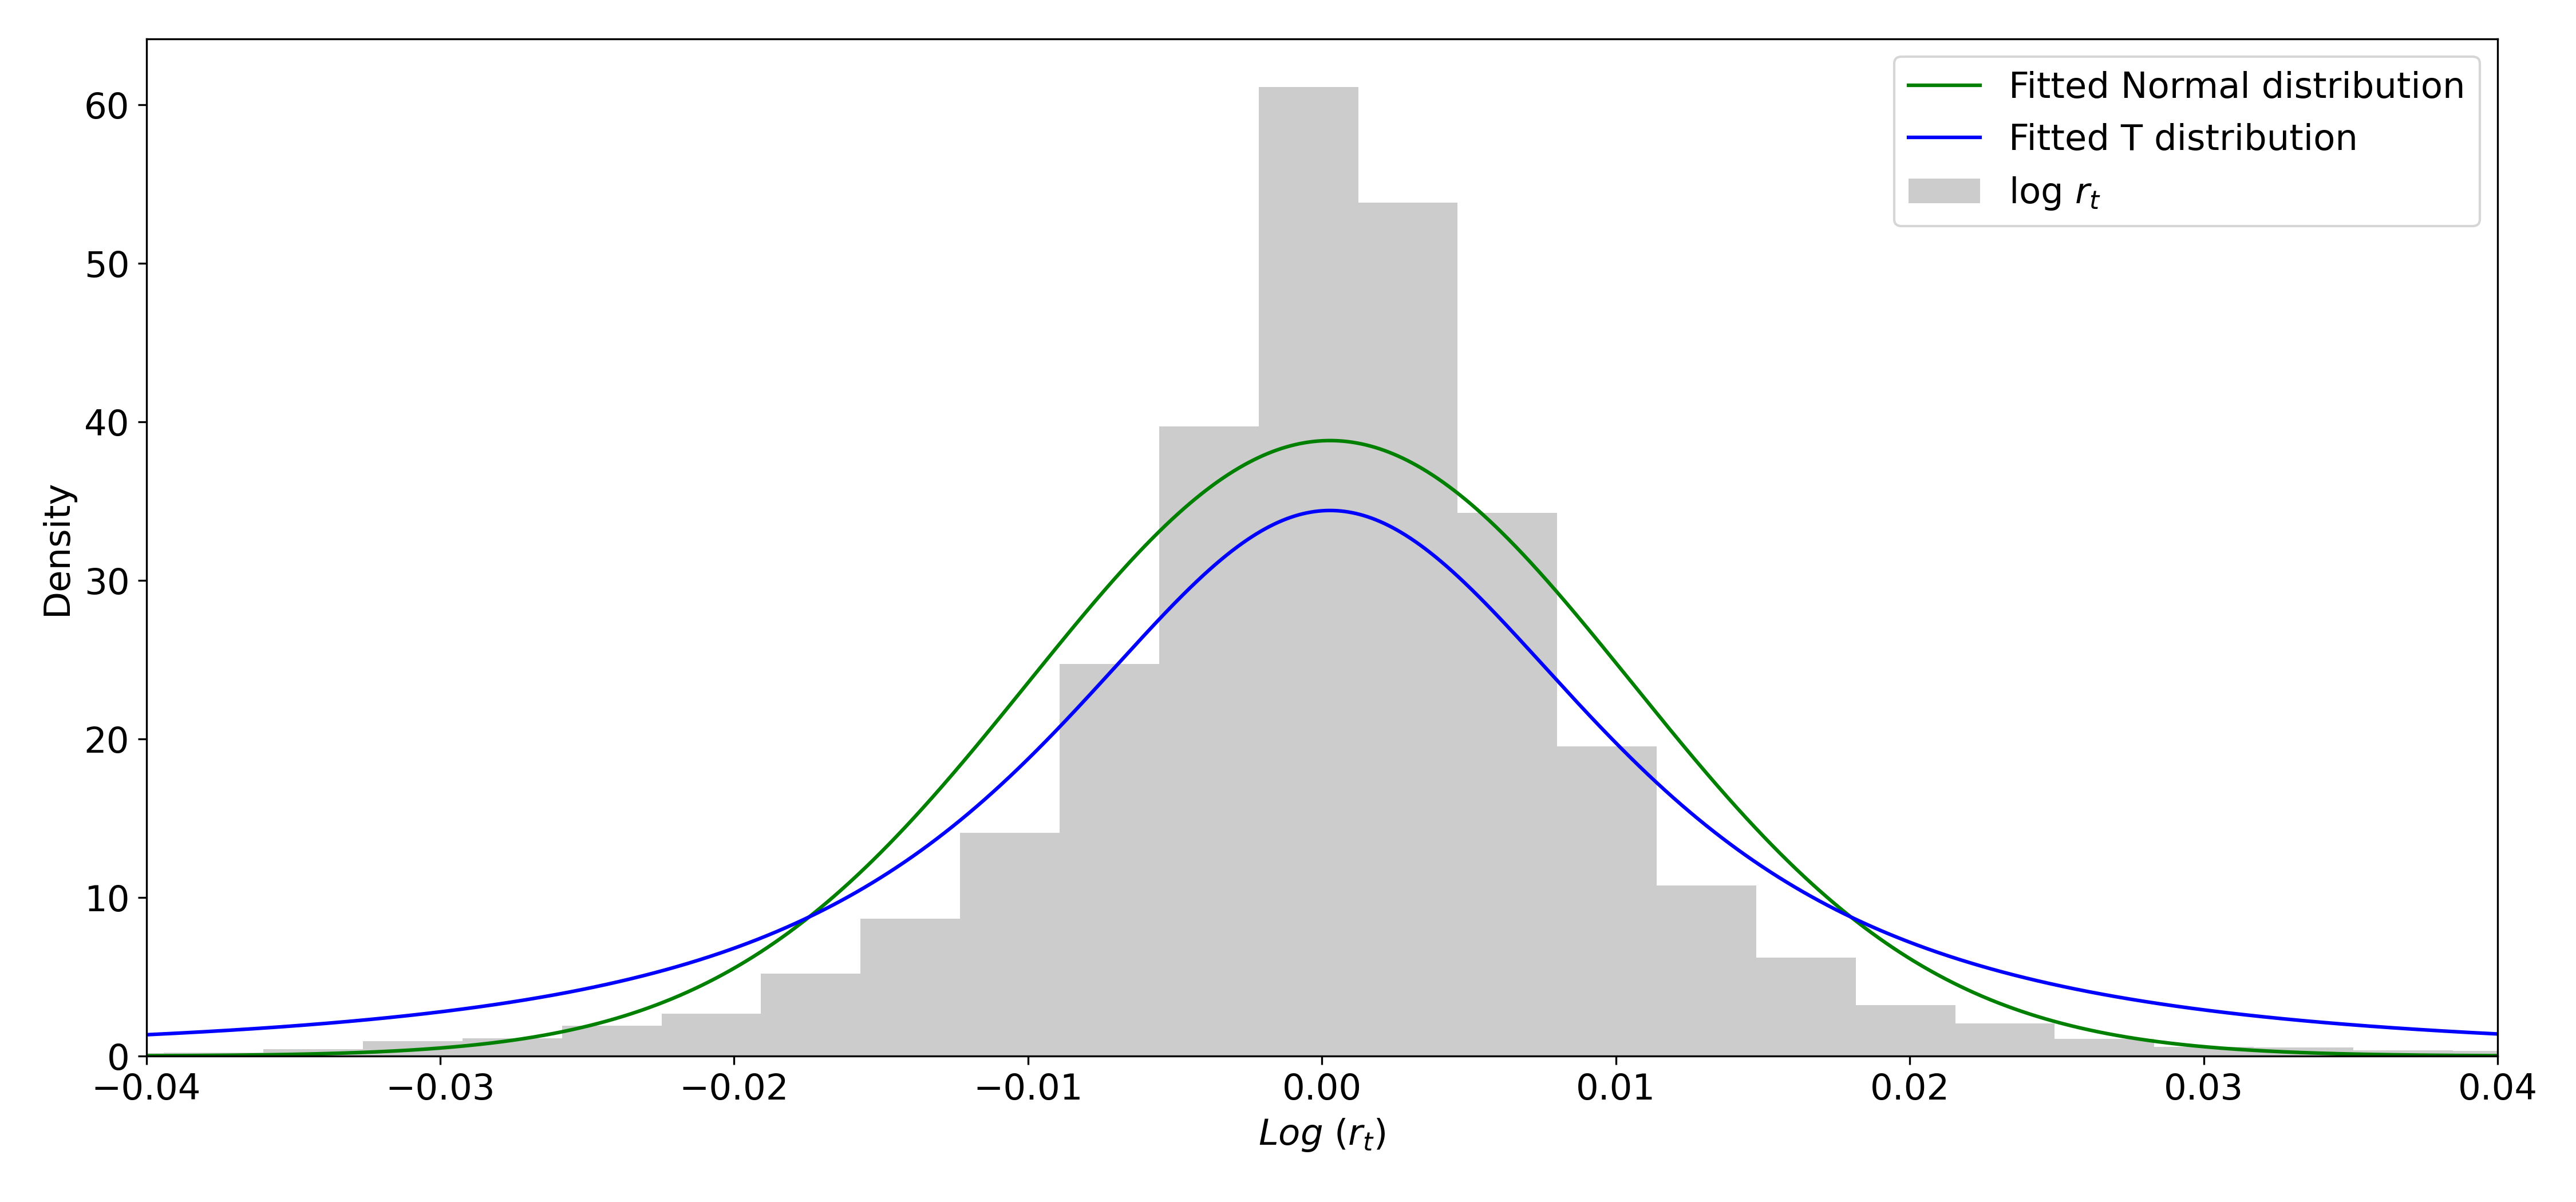
\includegraphics[width=1\textwidth]{analysis/data_description/images/SP500_distribution.png}
    \caption[Density plot of the S\&P 500 log returns] {Density plot of the S\&P 500 log returns. The gray bars highlights the empirical distribution, the blue curve is the fitted Gaussian distribution and the orange curve is the fitted T-distribution with 2.97 DF.}
    \label{fig: Kernel_distributions}
\end{figure}

Given the evident distributional properties from figure \ref{fig: Kernel_distributions}, an interesting analysis would be to uncover how many observations that lie more than 3 standard deviations from the mean. In total there are 219 observations that lie more than 3 standard deviations away from the mean which is way above the expected 46 if the series followed a Gaussian distribution. \textbf{Skriv formel i fodnote.} Out of these, 108 observations are located in the right side of the tail while the remaining 111 are located in the left tail. This phenomenon that large drawdowns occur more often than similar large upwards movements is well researched and known as the gain/loss asymmetry (Cont, 2001). In addition, it should be noted that since the S\&P 500 index contains 15,385 observations, it only takes a few outliers to reject that the series follows a Gaussian distribution. However, as noted by Cont (2001), financial returns are characterised by a large degree of extreme observations compared to the Gaussian distribution, hence the results are in line with expectations.


\textbf{Hvad er pointen med det her? Der er kun meget løst blevet talt om extreme observations vs. outliers, men det er hverken nærmere defineret eller bundet op på det underliggende data. TBD.}
Lastly, it is important to note the subtle distinction between outliers and extreme observations since extreme observations deviate considerably beyond 3 standard deviation from the mean, yet they may still hold meaningful information. Since extreme events happen in live markets the observation that they create should be included in the model estimation procedure in order for the model parameters to be as realistic as possible. The other side of the argument is that depending on the extremeness of the observations, they could potentially have severe impact on the parameter estimation resulting in the parameters being miss-specified, thereby serving as an argument for disregarding the extreme observations (Nystrup, 2014). These considerations will be further examined throughout section \ref{Section: Simulation study} and \ref{Section: Stylized facts}


\label{subsection: distributional properties}

\subsection{Temporal properties}
\label{subsection: temporal properties}
In addition to the aforementioned distributional properties, Granger \& Ding (1995b) as well as Cont (2001) further found that financial returns are characterised by a set of temporal properties. As such, it is evident by the plot in figure \ref{fig: log_returns_all_indices} that the log returns series is more volatile in some periods, for instance during Black Monday in 1987 since the log returns bounces between being highly negative and highly positive in a short period of time. The effect that large price movements tend to be followed by other large price movements, but not necessarily in the same direction, is known as volatility clustering and it is one of the stylized facts that is hardest for mathematical models to reproduce (Cont, 2001). However, it has been proven that regime-switching models replicate the absence of linear autocorrelation and the long-term memory property of the absolute autocorrelation function well, although simple regime-switching models struggle to achieve a simultaneous fit of the entire set of stylized facts (Rogers \& Zhang, 2011). Further analysis of this will be conducted in section \ref{Section: Stylized facts}, in which the thesis aims at achieving a simultaneous fit of the stylized facts defined by Granger \& Ding (1995b) through different estimation procedures of HMMs.

It is particularly evident from figure \ref{fig: log_returns_all_indices} that the S\&P 500 index appears to have increasing volatility through time. This is not a surprising finding since the S\&P 500 index includes observations from the 1960s. During these early days of the financial market, there were no active derivative markets and much fewer actors had direct access to trading financial instruments. As such, markets were simpler, less risky and thus characterised by an overall lower level of volatility compared to the past 40 years of development.

\begin{figure}[H] 
    \centering
    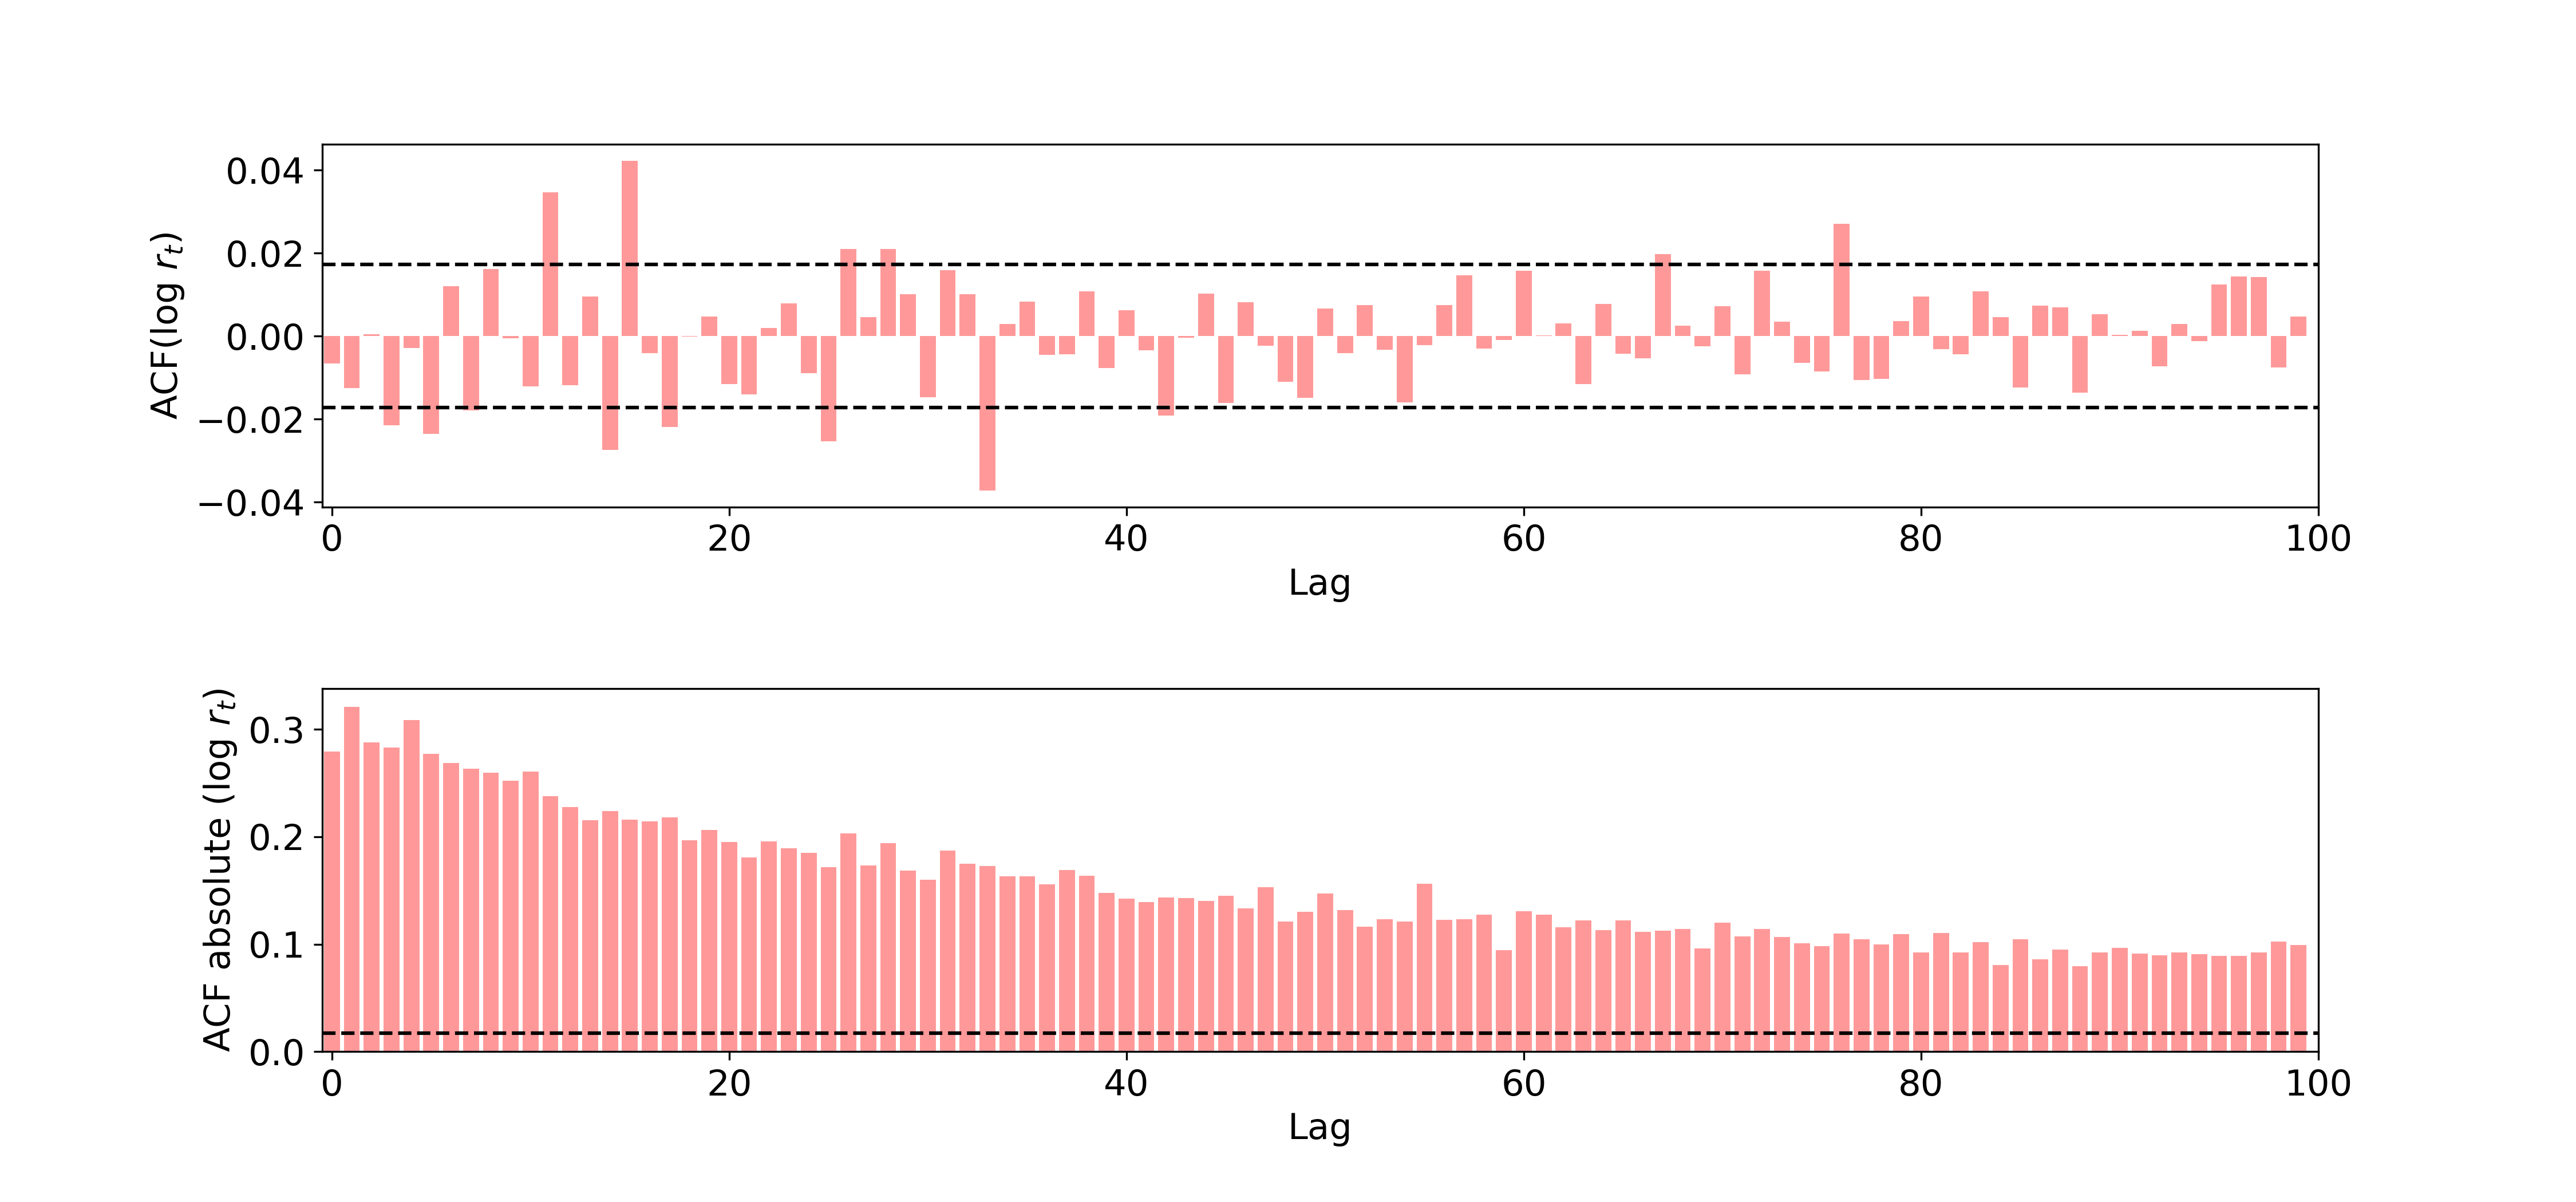
\includegraphics[width=1\textwidth]{analysis/data_description/images/SP500_ACF.png}
    \caption[ACF and absolute ACF for the S\&P500]{ACF and absolute ACF for the S\&P500. The dashed black lines represent the 95\% significance level. \textbf{Notation skal følge den i afsnit 6. Dvs log returns skrives ikke som $\log r_t$ og for absolutte returns skal der stå $ACF(|r_t|)$.}}
    \label{fig: ACF_all_log_returns}
\end{figure}

The autocorrelation function (ACF) for the log returns and the absolute log returns are shown in figure \ref{fig: ACF_all_log_returns}. As such, it is evident that the vast majority of the first order linear autocorrelation, at different lags, appears to be non-significant which is in accordance with the empirical studies conducted by Granger \& Ding (1995b) as well as Cont (2001). The fact that some of the lags are significant comes at no surprise either since, as previously discussed, large historical market events such as Black Monday could trigger significant linear autocorrelation, however, this is clearly not persistent across time. Contrary, the absolute ACF of the log returns is significant all the way up to around lag 450. This suggests that financial returns exhibit a long memory component, thereby making volatility somewhat predictable. As such, the long memory of the absolute log returns is closely related to the previously described volatility clustering from figure \ref{fig: log_returns_all_indices}. This finding is also congruent to the aforementioned empirical studies. Having introduced the data that will be used to estimate the HMMs as well as its distributional and temporal properties, the following section will briefly introduce the notation as well as some of the prominent literature associated with HMMs.

\subsection{Computing portfolio returns}

\textbf{TO be deleted}

\textbf{Add formulas for shorting costs and transaction costs here.}

Using the weights estimated at time t, the portfolio returns are calculated each day as the product of all assets' gross return and their respective weights.
\begin{equation}
    r_{t,portfolio} = \sum_{i=1}^N \left(w_{t,i}\times(1+r_{t,i})\right)  - 1
\end{equation}
Where, $r_{t,portfolio}$ is the portfolio return for day $t$ and $r_{t,i}$ \& $\pi_{t,i}$ denotes the return and weight of asset $i$ at day $t$. The weights are updated accordingly by the end of each day to reflect returns. The result is a series of portfolio returns with length equal to the amount of days in the sample. Total return over the period is then the product of all daily portfolio returns over the period
\begin{equation}
    r_{total} = \prod_{t=1}^T (1+r_{t, portfolio} ) - 1
    \label{eq:total_ret}
\end{equation}
\begin{equation}
    r_{annual}=(1+r_{total})^{1/T}-1
    \label{eq:annual_ret}
\end{equation}

\subsection{The MSCI}
\label{subsection: MSCI Index}
The MSCI World Index captures large and mid cap representation across 23 Developmed Markets (DM) countries. As such, the difference compared to the well-known MSCI ACWI Index is the exclusive weight on assets from developed economies. With 1,600 constituents, the index covers approximately 85\% of the free-float-adjusted market captilization in each country. The weights across country and sectors are shown in figure XXXXY as of November 2020. The historical development of the index is depicted in figure \ref{fig:MSCI_index}. 
 
\begin{figure}[H] 
    \centering
    
\includegraphics[width=1.0\textwidth]{analysis/data_description/images/MSCI_index.png}
    \caption{Development MSCI.}
    \label{fig:MSCI_index}
\end{figure}

%##### INDSÆT FIGUR AF Sector og region focus ####### # VIS split

The inclusion of the MSCI World Index is based on the fact that it is a global index, and thus should capture the economics trends across geographies. As such, the thesis treats it as a baseline index in terms of uncovering economic-regimes. Although it is a world index, North America makes up almost 2/3 of the index, however, this makes sense from an economic perspective since the U.S. economy serves as a fundamental indicator of how the remaining world economy is progressing. Furthermore, the information technology sector is by far the largest sector in the index, since it accounts for approximately 22\% of the overall allocation as per figure XXXXX. It should be noted that the weights are a snapshot in time, hence they are constantly changing. 

\begin{table}[H]
\caption{Summary statistics for the daily MSCI log-returns.}
\centering
\begin{tabular}{c c c c c c c c c} 
\hline\hline
Observations & Mean & STD & Skewness & Excess Kurtosis & Min & Max & First ACF & Annual SR \\
\hline
12,941 & 0.0003 & 0.0087 & -0.6521 & 10.8819 & -0.1044 & 0.0909 & 0.1337 & 0.4854 \\
\hline
\end{tabular}
\label{tab:summary_stats_MSCI}
\end{table}

Table \ref{tab:summary_stats_MSCI} shows the first four central moments together with the minimum and maximum observation, the first-order autocorrelation and the annual Sharpe ratio (SR). The SR is the excess return per unit risk, i.e. the excess return divided by the standard deviation (SD). The first observations originates from 1969-12-31 and the final included observations is the date 2021-02-12. It appears that the daily log-returns for the MSCI World Index are negatively skewed and the distribution is also characterised by being highly leptokurtic as the excess kurtosis is positive. As such, the summary statistics indicate that the log return series for the MSCI World Index, are characterised by the set of stylized facts that are commonly associated with financial returns. The range of the observations has a span of 0.1953, thereby indicating that the index can change significantly in high-volatility periods.

\subsection{DAX 30}
\label{subsection: DAX 30}
The DAX is a blue chip stock market index comprising the 30 largest listed German companies. It is similar in nature to FTSE 100 and the Dow Jones Industrial Average. The index is included in the analysis in order to get an estimate for, whether the model parameters will change significantly when trained on the DAX as opposed to the aforementioned indexes. As such, the DAX becomes particularly interesting since its composition of a small number of firms and a restrictive geographical focus on Germany means that it might not necessarily represent the vitality of the economy as a whole. 

\begin{figure}[H] 
    \centering
    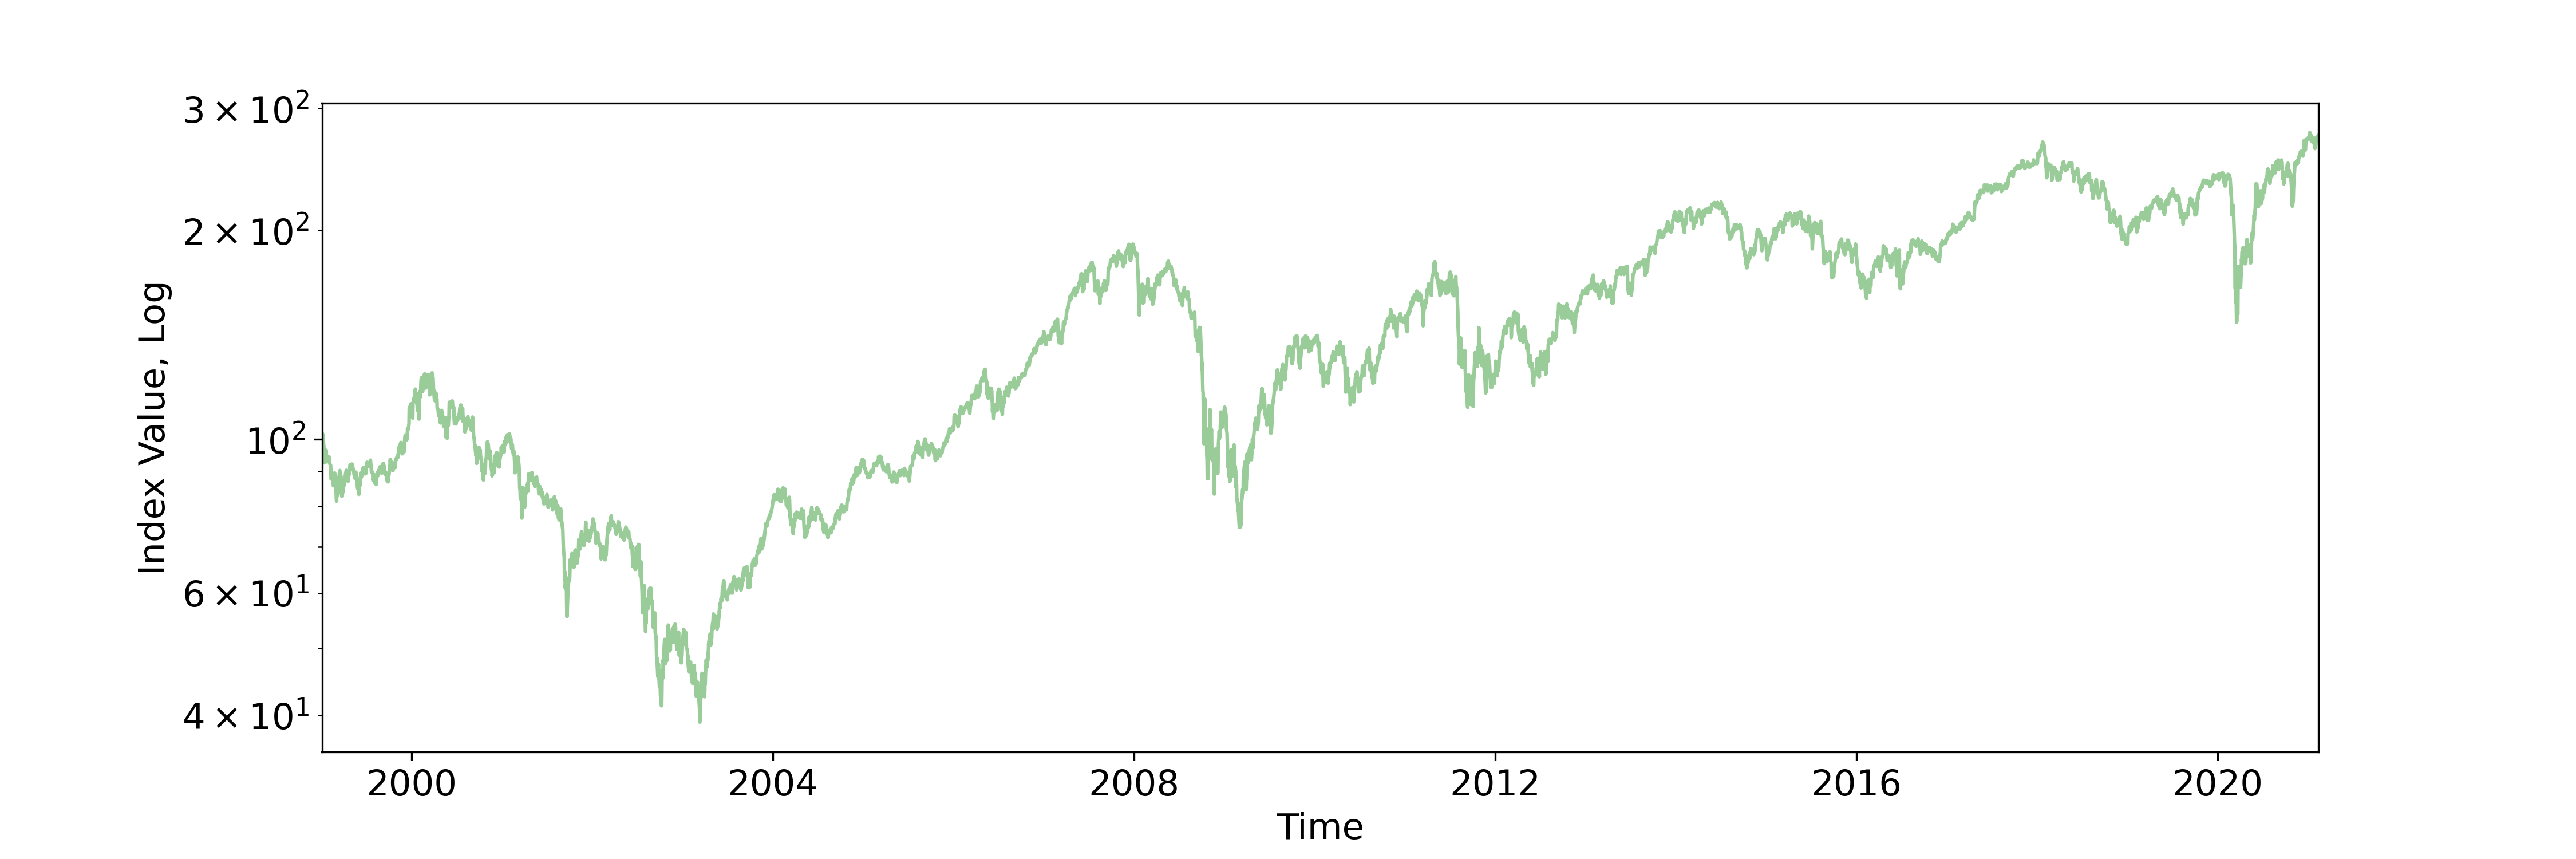
\includegraphics[width=1\textwidth]{analysis/data_description/images/DAX_index.png}
    \caption{Development DAX 30.}
    \label{fig: DAX_index}
\end{figure}

As is evident by figure \ref{fig: DAX_index}, the availability of daily data is significantly shorter compared to the MSCI World and the S\&P 500 Index. This is primarily due to the fact that the DAX 30 was originated in the late 1987. However, figure \ref{fig: DAX_index} also showcases that recent financial bear markets such as the dot-com bubble of the early 2000s, the GFC of 2008 as well as the COVID-19 rebound in Q1/Q2 2020 are well captured by DAX 30 Index. 

Since January 2006, the index is refreshed every second, however, the thesis will continue to rely on daily data frequencies as discussed in section \ref{subsection: Data frequency}. The index is capitalization-weighted and holds a total market capitalization of 1,017.7 billion EUR as of 21st of September 2020. In response to the recent accounting scandal related to Wirecard, Deutshce Börse announced an expansion of the DAX 30 to include 40 members. The expansion is set to occur in the third quarter of 2021.

\begin{table}[H]
\caption{Summary statistics for the daily DAX log-returns.}
\centering
\begin{tabular}{c c c c c c c c c} 
\hline\hline
Observations & Mean & STD & Skewness & Excess Kurtosis & Min & Max & First ACF & Annual SR \\
\hline
5,613 & 0.0002 & 0.0159 & -0.1869 & 2.8115 & -0.1394 & 0.1257 & 0.0146 & 0.1839 \\
\hline
\end{tabular}
\label{tab:summary_stats_DAX}
\end{table}

As highlighted by table \ref{tab:summary_stats_DAX}, the DAX Index contains much fewer observations compared to the MSCI World and S\&P 500 index. Furthermore, the DAX has similar mean daily returns although the standard deviation is the highest among the selected indices. However, the DAX is less negatively skewed and exhibit the lowest degree of leptokurtotic among the selected indexes. However, the high standard deviation naturally leads to a much lower Sharpe Ratio compared to the other indices at 0.1839.


##### Disitrbutional properties section:

The MSCI World Index appears to have a more stable trajectory with less volatile movements both compared to the S\&P 500 and the DAX 30. Despite this, the MSCI World Index generally trended in the same direction as the S\&P 500,
but in some periods the range between the two indices widened. For example,
it appears that the MSCI World and S\&P 500 Index trended in close correlation in the period from 1999 to 2015, however, from 2015 to 2021 the two indices have drifted apart. Furthermore, it appears that the S\&P 500 has become increasingly more volatile over the period 2015-2021, particularly evident by the recent COVID-19 rebound in which the drawdown of the S\&P 500 was much more extreme compared to the MSCI World.  

The DAX 30 performed particularly well in the period following the dot-com bubble, however, during 2008 and 2009 the GFC severely impacted the index, thereby bringing it down to the respective levels of the S\&P 500 and MSCI World. As concluded in section \ref{subsection: DAX 30} the DAX was characterised as the most volatile, which is also evident by figure \ref{fig: all_indices_index} which showcases that the DAX indeed appears to have a higher volatility. From 2006 to 2017 the DAX Index has consistently been at higher index levels compared to the other indices until the S\&P 500 caught up by breaking its all time high in 2019. An overview of the summary statistics for each index is listed in table \ref{tab:summary_all}.

#### LAst comment temporal properties

Conclusively, the reader should note that the correlation among the indices are stronger at the times of high market volatility. This is perhaps not surprising since the indices are made up of stocks, however, it highlights that diversification based on investing in different sectors or geographical areas may not materialize precisely when an investor needs it the most. The impact would most probably be less significant if one were to compare a stock index with a bond index, since the correlation would be lower, especially during periods of high volatility. Despite the fact that correlations increased in high volatility markets, there are definitely benefits related to diversification between asset classes.